\chapter{Simulação Distribuída}


\section{Time Warp}
	Um dos mais conhecidos protocolos otimistas é o Time Warp, que possui algumas implementações, tais como \textit{Jade Time Warp} \cite{BAEZNER1}, o sistema \textit{SPEE-DES} (\textit{Synchronous Parallel Environment for Emulation and Discrete Event Simulation})\cite{STEINMAN92}, o \textit{WARPED} \cite{WARPED} e o \textit{Georgia Tech Time Warp (GTW)} \cite{DAS94}. O \textit{Time Warp} foi originalmente proposto por Jefferson(1995). 
	Basicamente, o \textit{Time Warp} trata os erros de causa e efeito por meio de duas estruturas internas:
\begin{itemize}
	\item O controle local, que é interno a cada processo organizando os eventos para que sejam executados em ordem cronológica.
	\item O controle global, destinado ao cálculo do \textit{GVT}(\textit{Global Virtual Time}). 
\end{itemize}

%% Realmente muito estranho
	%Por organizar os eventos em ordem cronológica, internamente o \textit{Time Warp} se assemelha a um protocolo de simulação sequencial. Porém, há diferenças básicas entre ambos, como cada processo do \textit{Time Warp} pode resultar de outros processos dentro da simulação, e também após o cálculo do \textit{GVT} os processos com tempos inferiores à este são descartados.

	%São feitas cópias internas às estruturas dos estados dos processos para a realização do \textit{rollback}. Viabilizando a execução do \textit{rollback} quando uma mensagem com \textit{timestamped} com tempo inferior ao \textit{LVT} do processo atual, assim interrompendo o processamento e daí recuperando  o estado imediatamente anterior ao timestamped, envia novamente as mensagens da lista de saída, sinalizando aos respectivos processos que aquelas mensagens estão incorretas e não devem ser consideradas.

\subsection{Mensagem}
Mensagens são as informações trocadas entre os processos durante a simulação. E quando se trata de uma troca de mensagens entre processos, ela é marcada com o tempo no qual o evento que ela representa deva ser processado, (\textit{timestamped}).
A lista de eventos é organizada em ordem cronológica do seu tempo lógico e as mensagens que geraram estes eventos são denominadas mensagens positivas. Os eventos que já foram processados são mantidos em uma lista, denominada lista de saída de mensagens. Essas mensagens contêm uma marca de tempo menor ou igual ao \textit{LVT} do processo, visto que já foram processadas, e são denominadas mensagens negativas ou anti-mensagens. Essa lista só é utilizada se for necessária a realização de \textit{rollbacks}.

\subsection{Anti-Mensagem}%%%%%%% Falta-me conceito, esqueci já.
Para ocorrer um \textit{rollback} é necessário o retorno dos processos aos seus estados anteriores, isto ocorre quando chega uma mensagem \textit{strangler}. E, para os demais processos serem avisados do \textit{rollback}, as anti-mensagens são enviadas aos processos que devem retornar aos seus estados anteriores.

\subsection{Sincronização}
Novas soluções para garantir o sincronismo dos eventos em um sistema distribuídos vêm sendo desenvolvidos ao longo dos anos, tendo em vista o grande aumento da utilização desse tipo de sistema. A eficiência de um sistema distribuído está diretamente ligado à sua capacidade de sincronizar os eventos adequadamente, garantindo que o mínimo de recurso e de tempo seja despendido para a realização dos processos de recuperação e que o resultado final seja consistente.

	Para garantir a consistência do resultado de uma simulação, deve-se respeitar a regra de causa e efeito, ou seja, deve-se garantir que nenhum evento $e_b$ ocorra antes de um evento $e_a$ qualquer, sendo $a<b$.
	
	Em um protocolo otimista, a solução se dá em guardar os dados referentes aos eventos anteriores caso haja a necessidade de se retornar à um tempo anterior ao atual, devido a falha de causa e efeito. 
	
	O sistema deverá ser capaz de retornar a uma situação anterior ao tempo da referida mensagem, e garantir que todos os eventos processados com \textit{LVT} maior que o da mensagem sejam desfeitos. A imagem a seguir ajuda a ilustrar a ocorrência de uma mensagem s\textit{trangler} :

\begin{figure}
  \centerline{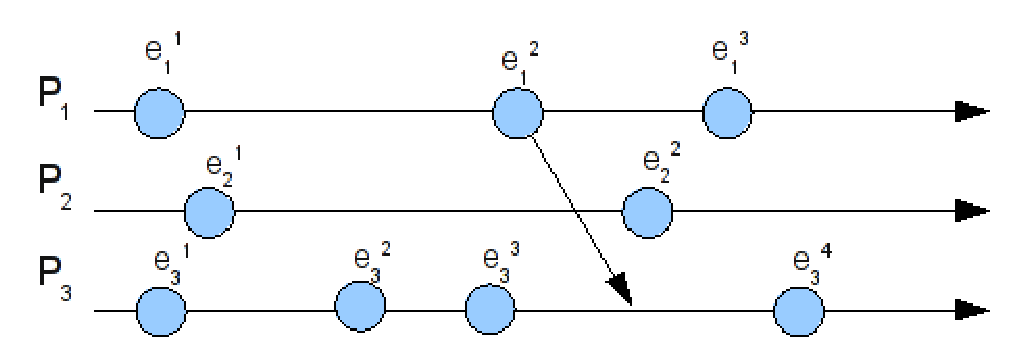
\includegraphics[scale=0.6]{strangler.eps}}
  \caption{Mensagem strangler.}
\label{fig:strangler}
\end{figure}

	No exemplo acima, o processo $e_{12}$ envia uma mensagem com \textit{LVT} igual a 2 para um processo que já está no tempo 3. Isso gera uma mensagem \textit{straggler}, pois o evento $e_{33}$ só deveria ser executado após o recebimento da mensagem. Para a correção, o protocolo deve garantir que o evento $e_{33}$ seja desfeito e que ele somente seja executado depois do do recebimento da mensagem enviada pelo evento $e_{12}$.
	Em sistemas distribuidos, onde não há uma área de memória comum à todos os processos, faz-se necessário a utlização de algumas técnicas que garantam que a observação remota do sistema não seja incompleta ou inconsistente, uma vez que os eventos se alternam com frequência e não existe um relógio global de referência.
	
\subsection{Estados Locais e Estados Globais}
Para se compor o quadro completo de uma simulação distribuída (estado global)  este quadro a partir de diversos pequenos quadros (estados locais). Cada um dos $k$ eventos de um processo $p_i$ são representados por $e_{ki}$.
\begin{itemize}
	\item \textbf{Estado local} - Um estado local $ \sigma_{ki} $ é definido como sendo os valores das variáveis do processo pi após a execução de seu evento $e_{ki}$.
	Estendendo esta definição para o estado globlas:


	\item \textbf{Estado Global} -  O estado $\Sigma$ é o conjunto de $n$ estados locais, sendo $n$ o número de processos, e cada um dos $n$ elementos o estado local de um processo. Assim, $ \Sigma = (\sigma_1, \sigma_2, \sigma_3, ..., \sigma_n)$.
\end{itemize}


	Percebe-se que partindo das definições de estados locais, que contém os valores das variáveis de um processo após a execução de um evento, e de estado globais, que é o conjunto de estados locais, possuí aí então um retrato da simulação em um tempo $t$ qualquer.

\subsection{Cortes Globais Consistentes}
Um corte em um sistema distribuído é um conjunto C de seus eventos executados. Denominamos fronteira de corte o conjunto que contém os últimos eventos de cada processo. A figura a seguir ilustra dois cortes dados pelos conjunto $C'\{e_{12}, e_{21}, e_{32}\}$ e $C''\{e_{12}, e_{22}, e_{33}\}$ :

	Um corte consistente é fechado à esquerda sobre a relação de precedência causal, ou seja, toda seta que intercepta o corte tem sua origem à esquerda.

	Ou seja, no corte $C'$, ilustrado acima, há um corte consistente. Porém no corte $C''$ percebe-se que uma mensagem foi recebida imediatamente anterior ao tempo 3 no processo P3, porém esta mensagem ainda não foi enviado, pois o evento que deveria te-lo feito está a direita do corte $C''$, ou seja, o evento ainda não ocoreu. Sendo assim, o corte $C''$ contém uma inconsistência.
	Da definição de corte consistente obtém-se o conceito de \textbf{Estado Global Consistente}, que corresponde a um corte global consistente. De um estado global consistente nota-se que se trata de um instante que não fere a sequência de causa e efeito da simulação, tratando-se entanto de um ponto seguro de retorno em caso de um futuro \textit{rollback}.
	
\begin{figure}
  \centerline{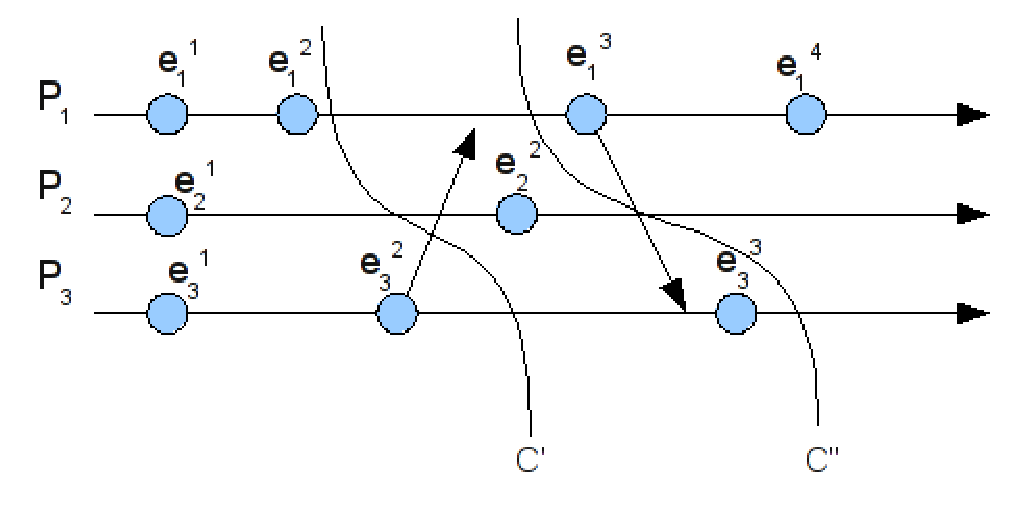
\includegraphics[scale=0.6]{cortes.eps}}
  \caption{Cortes.}
\label{fig:cortes}
\end{figure}
	
